\documentclass[12pt,a4paper]{article}
\usepackage[utf8]{inputenc}
% \usepackage[russian]{babel}
\usepackage[OT1]{fontenc}
\usepackage{color}
\usepackage{amsmath}
\usepackage{listings}
\usepackage{amsfonts}
\usepackage{amssymb}
\usepackage[pdftex]{graphicx}
\author{Bykov A.E.}
\usepackage{tikz}
%tikz library includes
\usetikzlibrary[arrows]
\usetikzlibrary[automata]
\usetikzlibrary[backgrounds]
\usetikzlibrary[calc]
\usetikzlibrary[calendar]
\usetikzlibrary[chains]
\usetikzlibrary[decorations]
\usetikzlibrary[decorations.footprints]
\usetikzlibrary[decorations.fractals]
\usetikzlibrary[decorations.markings]
\usetikzlibrary[decorations.pathmorphing]
\usetikzlibrary[decorations.pathreplacing]
\usetikzlibrary[decorations.shapes]
\usetikzlibrary[decorations.text]
\usetikzlibrary[er]
\usetikzlibrary[fadings]
\usetikzlibrary[fit]
\usetikzlibrary[folding]
\usetikzlibrary[matrix]
\usetikzlibrary[mindmap]
\usetikzlibrary[patterns]
\usetikzlibrary[petri]
%%\usetikzlibrary[placements]
\usetikzlibrary[plothandlers]
\usetikzlibrary[plotmarks]
\usetikzlibrary[positioning]
\usetikzlibrary[scopes]
\usetikzlibrary[shadows]
\usetikzlibrary[shapes.arrows]
%%\usetikzlibrary[shapes.callout]
\usetikzlibrary[shapes.gates.logic.US]
\usetikzlibrary[shapes.gates.logic.IEC]
\usetikzlibrary[shapes.geometric]
\usetikzlibrary[shapes.multipart]
\usetikzlibrary[shapes.multipart]
\usetikzlibrary[shapes.misc]
\usetikzlibrary[shapes.symbols]
\usetikzlibrary[through]
\usetikzlibrary[topaths]
\usetikzlibrary[trees]
\begin{document}
\definecolor{dkgreen}{rgb}{0,0.6,0}
\definecolor{gray}{rgb}{0.5,0.5,0.5} 
\lstset{ %
  language=Octave,                % the language of the code
  basicstyle=\footnotesize,           % the size of the fonts that are used for the code
  numbers=left,                   % where to put the line-numbers
  numberstyle=\tiny\color{gray},  % the style that is used for the line-numbers
  stepnumber=1,                   % the step between two line-numbers. If it's 1, each line 
                                  % will be numbered
  numbersep=5pt,                  % how far the line-numbers are from the code
  backgroundcolor=\color{white},      % choose the background color. You must add \usepackage{color}
  showspaces=false,               % show spaces adding particular underscores
  showstringspaces=false,         % underline spaces within strings
  showtabs=false,                 % show tabs within strings adding particular underscores
  frame=single,                   % adds a frame around the code
  rulecolor=\color{black},        % if not set, the frame-color may be changed on line-breaks within not-black text (e.g. comments (green here))
  tabsize=2,                      % sets default tabsize to 2 spaces
  captionpos=b,                   % sets the caption-position to bottom
  breaklines=true,                % sets automatic line breaking
  breakatwhitespace=false,        % sets if automatic breaks should only happen at whitespace
 % title=\lstname,                   % show the filename of files included with \lstinputlisting;
                                  % also try caption instead of title
  keywordstyle=\color{blue},          % keyword style
  commentstyle=\color{dkgreen}       % comment style
}
\newcommand{\happysmile}[1]{
\begin{tikzpicture}[scale=#1/10]
  \fill[yellow] (0,0) circle (2);
  \draw (0.75,0.5) circle (0.25);
  \draw (-0.75,0.5) circle (0.25);
  \draw (1,-0.5)..controls(0,-1.5)..(-1,-0.5);
\end{tikzpicture}
}
\newcommand{\sadsmile}[1]{
\begin{tikzpicture}[scale=#1/10]
  \fill[yellow] (0,0) circle (2);
  \draw (0.75,0.5) circle (0.25);
  \draw (-0.75,0.5) circle (0.25);
  \draw (1,-1)..controls(0,-0.5)..(-1,-1);
\end{tikzpicture}
}

\newcommand{\newtitle}[2]{
\title{#1}
\author{#2}
\maketitle
\tableofcontents
\pagebreak
}
\newcommand{\definition}[2]{
\underline{\textit{#1}}- #2
}
\newcommand{\code}[2]{
\lstinputlisting[caption={#2},label=DescriptiveLabel,language=Java]{samples/#1}
}
\newtitle{Technical Task}{Innopolis University,\\ autumn semestsr course project\\ Bykov Anton}
\section{Technical task for the Phase 1}
The objective of this phase is to utilize the database knowledge for real life problems.
\begin{enumerate}
\item Design the relational model and transform them into relations (create
ER diagram and translate it into Relations).
\item Design the relations in an existing database management system (DBMS) by creating physical tables and their relationships.
\end{enumerate}
\subsection{Creating Scheme}
There are many repositories containing research articles with their information.
\begin{figure}[h]
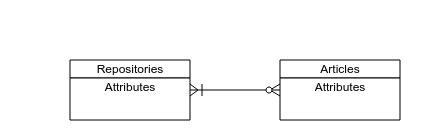
\includegraphics[scale=0.7891]{media/phase1/figure1.jpg}\\
\caption{The same article may be stored in different repositories.}
\end{figure}

The research articles are usually categorized based on their venues, authors, types and years.
\begin{figure}[h!]
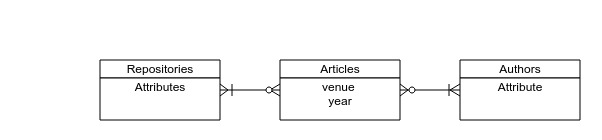
\includegraphics[scale=0.5791]{media/phase1/figure2.jpg}\\
\caption{The same article may be written by different authors.}
\end{figure}

A publication record reference in research articles can have several attributes along with the article name.\\
\begin{figure}[h!]
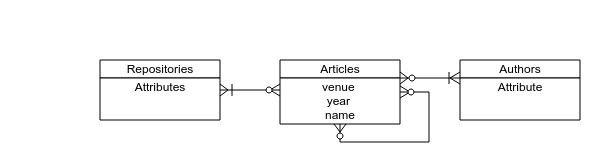
\includegraphics[scale=0.5791]{media/phase1/figure3.jpg}\\
\caption{The same article may be referenced in different articles.}
\end{figure}


Functionality:
\begin{itemize}
\item Select, Insert, delete, and update publication records
\item Import at least 1 million publications that are crawled from an existing publication repository, e.g. DBLP or Google Scholar, ACM digital
library or etc. Realtime crawling is a +.
\item Search the publication based on research area, author name, publi-
cation year, venue(conference/journal name), title, keyword, type of
paper, institution or related articles and obtained ordered results.
\item Ability to query related articles, based on your own defined methods,
\color{red}
at least two methods.
\color{black}
\item Ability to sort papers based on your own defined ranking methods, \color{red}at least two methods\color{black}
\end{itemize}
\subsection{Implementing scheme}
According to relations from 1.1, it is needed to implement a database on PostgreSQL
\section{Technical task for the Phase 2}
After creating the physical database, you need to develop a web-based graphical user interface (GUI) on top of it to interact with the database. It helps the users to carry out all the specified functionalities. It is more like Content Management System CMS. Only authorized/registered users are allowed to use this interface.

The web interface must neatly report the results with ranking. A nice visualization of the results, like showing graphs for related articles, is a +.

\section{Technical task for the Phase 3}
The goal of this phase is to replace the relational database with your own implementation of a database. You are asked to implement query operators (scan, select, project, join, group by, insert) using a standard programming language. You will replace all SQL code with calls to the query operators.
Note that from the user’s point of view, nothing will change on the front end insert) side of your web application. These are the requirements of the third phase of the project:
\begin{itemize}
\item Your database must provide methods to query data, as well as insert new record and update existing records.
\item Your database should provide methods to query data, as well as insert new record and update existing records.
\item In particular, your database should at least answer queries that join two tables.
\item Use the iterator model to implement query operators. That is, operators should pull tuples from underlying operators using next() calls.
\item Indexing on Primary keys with ability to add index on other attributes.
\end{itemize}
\end{document}